

% \begin{frame}[t]{AER: Challenges and Contribution}

% %   \begin{columns}[T,onlytextwidth]

% %     \column{0.45\textwidth}
% %     \begin{block}{State Of The Art}
% %     \begin{enumerate}
% %         \item discrete (sparse) SIMO BCE
% %         \\based on time-domain XREL
% %         \item Peak-picking
% %     \end{enumerate}
% %     \end{block}

% %     \column{0.45\textwidth}
% %     \only<2,3>{
% %         \begin{block}{$\implies$ however}
% %             \begin{itemize}
% %                 \item Estimation in the RIR space
% %                 \\memory issue
% %                 \item Echoes are ``off-grid''
% %                 \\accuracy issues and mismatch
% %                 \item Peak picking and labeling
% %                 \\tuned and NP-hard
% %             \end{itemize}
% %         \end{block}
% %     }

% %     \end{columns}

% %     \vspace{1em}

%     \begin{alertblock}{$\implies$ we propose}

%     \vspace*{.5em}
%     \begin{columns}[T, onlytextwidth]
%         \column{0.45\textwidth}
%         \blaster {\small \cite{di2020blaster}}
%         \begin{enumerate}
%             \item Knowledge-based approach
%             \item BCE + Continuous Dictionary
%             \\based on XREL
%             \item Iterative-like approach
%             \item Inputs:
%             \begin{itemize}
%                 \item stereo mic recordings
%                 \item \# echoes
%             \end{itemize}
%             \item Output: $\set{\tau_i^{(r)}, \alpha_i^{(r)}}_{i,r}$
%         \end{enumerate}

%         \column{0.45\textwidth}
%         \lantern {\small \cite{di2019mirage}}
%         \begin{enumerate}
%             \item Learning-based regression
%             \item Deep Learning used for SSL
%             \item Inputs: stereo audio feature
%             \item Output in the TDOA space
%             \\($\neq$ Echo space)
%         \end{enumerate}
%     \end{columns}
% \end{alertblock}

% \end{frame}



\begin{frame}{AER as discrete SIMO BCE {\hfill\small (common knowledge)}}

    \begin{block}{Key ingredient -- \textit{Cross relation identity}}

        \vspace{-3mm}
        \begin{columns}[onlytextwidth]
        \column{0.6\textwidth}
            \begin{align*}
                \contMic_1 &= \contRIR_1 \contConv \contSrc
                \\\contRIR_2 \contConv \contMic_1 = \textcolor{gray}{\contRIR_2 \contConv \contRIR_1 \contConv \contSrc}
                    &\textcolor{gray}{= \contRIR_1 \contConv \contRIR_2 \contConv \contSrc} = \contRIR_1 \contConv \contMic_2
                % \\\only<1>{\contRIR_2 \contConv \contMic_1 &= \contRIR_1 \contConv \contMic_2}
                %   \only<2->{\contRIR_2 \contConv \contMic_1 &- \contRIR_1 \contConv \contMic_2 = 0}
            \end{align*}

            \column{0.3\textwidth}
            \centering
            \only<1>{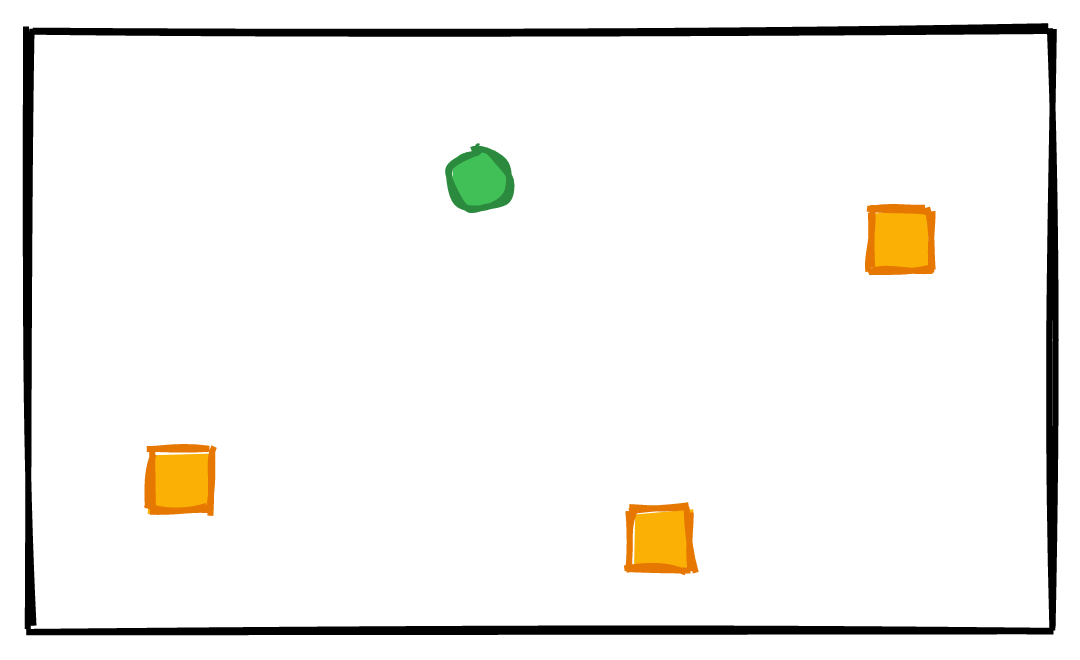
\includegraphics[width=0.9\textwidth]{figures/xrelation1.png}}%
            \only<2->{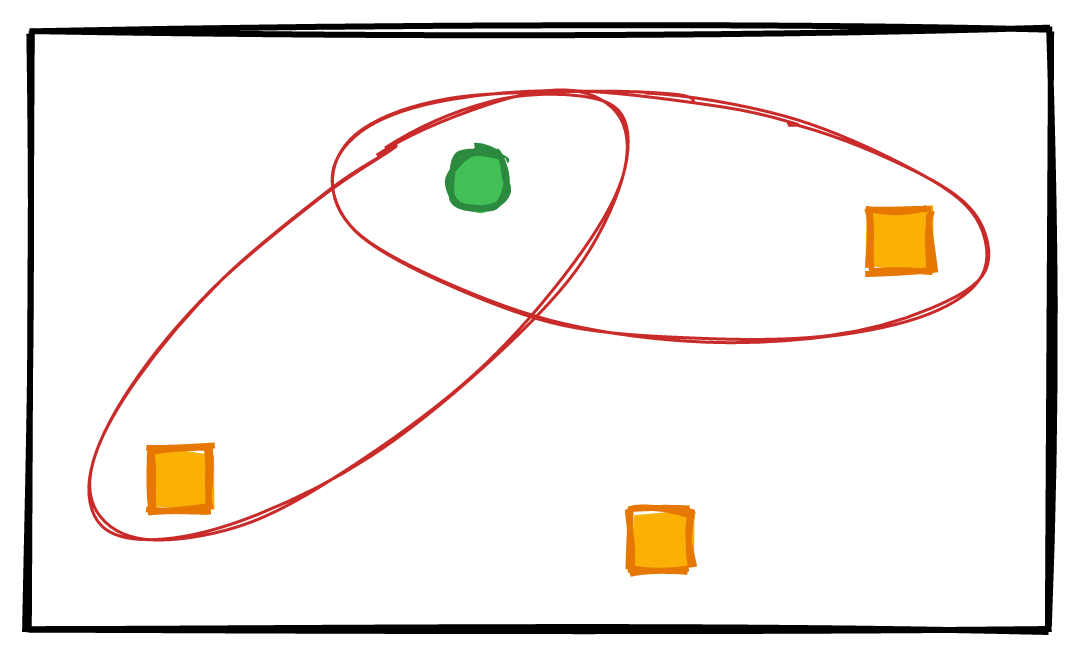
\includegraphics[width=0.9\textwidth]{figures/xrelation2.png}}
        \end{columns}
    \end{block}

    \vfill
    \begin{block}{Ideas:}
    \begin{enumerate}
        \small
        \item[\faCreativeCommonsSamplingPlus] Sampled version of $\contMic_1,\contMic_2$ are available ($\discMic_1, \discMic_2$)
        \item Echoes' $\tauir$ $\propto$ sampling frequency
        \item Find echoes $\rightarrow$ \textbf{find sparse vectors} $\discRIR_1, \discRIR_2$ of length $L$
        \item Modeled as \textbf{Lasso}-like problem

        \vspace*{.25em}
        \begin{mysotablock}
            \begin{equation*}
                \widehat{\discRIR}_1, \widehat{\discRIR}_2 \in
                \underset{\discRIR_1, \discRIR_2\in\kR^n}{\arg\min}\;
                \Vert \discMic_1 \contConv \discRIR_2 - \discMic_2 \tikzmarknode{conv}{\contConv} \discRIR_1 \Vert_2^2
                + \lambda \mathcal{P}(\discRIR_1, \discRIR_2)
                \quad\text{s.t.}\quad\mathcal{C}(\discRIR_1, \discRIR_2)
            \end{equation*}

            \vspace*{-2mm}
            \begin{center}
                \footnotesize
                $\mathcal{P}(\discRIR_1, \discRIR_2)$ $\longrightarrow$ sparse promoting regularizer
                \hspace{5mm} \footnotesize $\mathcal{C}(\discRIR_1, \discRIR_2)$ $\longrightarrow$ constraints e.g. \parbox{6em}{nonnegativity\\anchor}
            \end{center}
        \end{mysotablock}

    \end{enumerate}
    \begin{tikzpicture}[overlay,remember picture, %
        nodes={inner sep=1pt, align=center, color=gray, font=\footnotesize}, %
        gray,>=stealth] %
    \draw[->] (conv.north) to[out=90, in=180] ++ (+10mm,+4mm) node[right] %
        {{= $\mathtt{Toeplitz}(\discMic_i) \discRIR_j \in \mathcal{O}(L^2)$}};
    \end{tikzpicture}
    \end{block}

    \begin{center}
        \footnotesize
        \textcolor{mygreen}{\cmark}  \cite{tong1994blind} \qquad \textcolor{mygreen}{\cmark}  \cite{lin2008blind} \qquad \textcolor{mygreen}{\cmark} \cite{aissa2008blind} \\
        \textcolor{mygreen}{\cmark} \cite{kowalczyk2013blind} \qquad \textcolor{mygreen}{\cmark} \cite{crocco2015room,crocco2016estimation}
    \end{center}

 \end{frame}



% \begin{frame}{\blaster - Knowledge-based Off-grid AER}

%     \begin{block}{\textbf{Observation 1:} the cross relation remains true in the frequency domain}
%         \begin{equation*}
%             \mathcal{F}x_1 \cdot \mathcal{F}h_2 (\sfrac{n}{F_s}) = \mathcal{F}x_2 \cdot \mathcal{F}h_1(\sfrac{n}{F_s}) \qquad n=0\dots N-1
%         \end{equation*}
%         \end{block}

%         \vspace{.5em}

%         \pause
%         \begin{block}{\textbf{Observation 2:} $\mathcal{F}\delta_{\mathrm{echo}}$ is known in closed-form}
%         \end{block}

%         \pause
%         \vspace{1.em}
%         \begin{block}{\textbf{Observation 3:} $\mathcal{F}{\mathrm{x_i}}$ can be (well) approximated by DFT}
%         \begin{equation*}
%             \mathbf{X}_i = \texttt{DFT}(\discMic_i) \simeq  \mathcal{F}{\discMic_i}(nF_s) \qquad n=0\dots N-1
%         \end{equation*}
%         \end{block}


%         \pause
%         \vfill
%         \setbeamercolor{block title}{fg=white,bg=darkblue}
%         \setbeamercolor{block body}{fg=black,bg=bluegreen!10}
%         \begin{block}{\textbf{Idea:} Recover echoes by matching a finite number of frequencies}
%         \begin{equation*}
%             \underset{h_1,h_2 \in \substack{\text{measure} \\ \text{space}}}{\arg\min} \;
%             \tfrac{1}{2} \kvvbar{
%                 \mathbf{X}_1 \cdot \mathcal{F}h_2 (f) - \mathbf{X}_2 \cdot \mathcal{F}h_1(f)
%             }_2^2
%             + \lambda \kvvbar{h_1 + h_2}_{\mathrm{TV}}
%             \quad
%             \text{s.t.}\;
%             \begin{cases}
%                 h_1(\{0\})=1 \\
%                 h_l \geq 0
%                 \end{cases}
%         \end{equation*}
%         \end{block}

%         \pause
%         \begin{center}
%             $\sim$ \textbf{Lasso} problem, but $\mathcal{F}h_2 (f)$ is a continuous function.
%             \\Instance of a \textbf{BLasso} problem~\cite{bredies2020sparsity}
%             \\Solved with Sliding Frank-Wolfe algorithm \cite{denoyelle2019sliding}
%         \end{center}

%         \begin{center}
%             \textcolor{mygreen}{\cmark{no Toeplitz matrix} \qquad
%             \cmark \, \parbox{8.5em}{Solutions is \\ a train of Dirac} \qquad
%             \cmark \, \parbox{8em}{anchor prevents \\ trivial solution}}
%         \end{center}

%         % In the manuscript:
%         % \begin{itemize}
%         %     \item From Lasso to BLasso
%         %     \item Pseudocode of the Algorithm
%         %     \item How to manually tuned lambda
%         % \end{itemize}
% \end{frame}

% \begin{frame}[t]{\blaster - Experimental Results}
%     % \begin{block}{Scenario}
%     %     \begin{itemize}
%     %         \item simulation data with ISM with Pyroomacoustics
%     %         \item 1 source, 2 microphones, random room geometry
%     %         \item Full RIRs
%     %         \item 2 sources: broadband and speech
%     %         \item 2 datasets: different SNR, different RT60
%     %     \end{itemize}
%     % \end{block}
%     \begin{columns}[onlytextwidth]
%         \begin{column}{0.45\textwidth}
%             \begin{block}{Methods}
%                 \begin{itemize}
%                     \item BSN --- SIMO BCE\cite{lin2007blind}
%                     \item IL1C: iteratively-weighted $\ell_1$ constraint SIMO BCE
%                     \\\cite{crocco2015room}
%                     \item \blaster: Proposed off-grid approach
%                 \end{itemize}
%             Baseline method are xvalidated on other dataset
%             \end{block}
%         \end{column}

%         \begin{column}{0.45\textwidth}
%             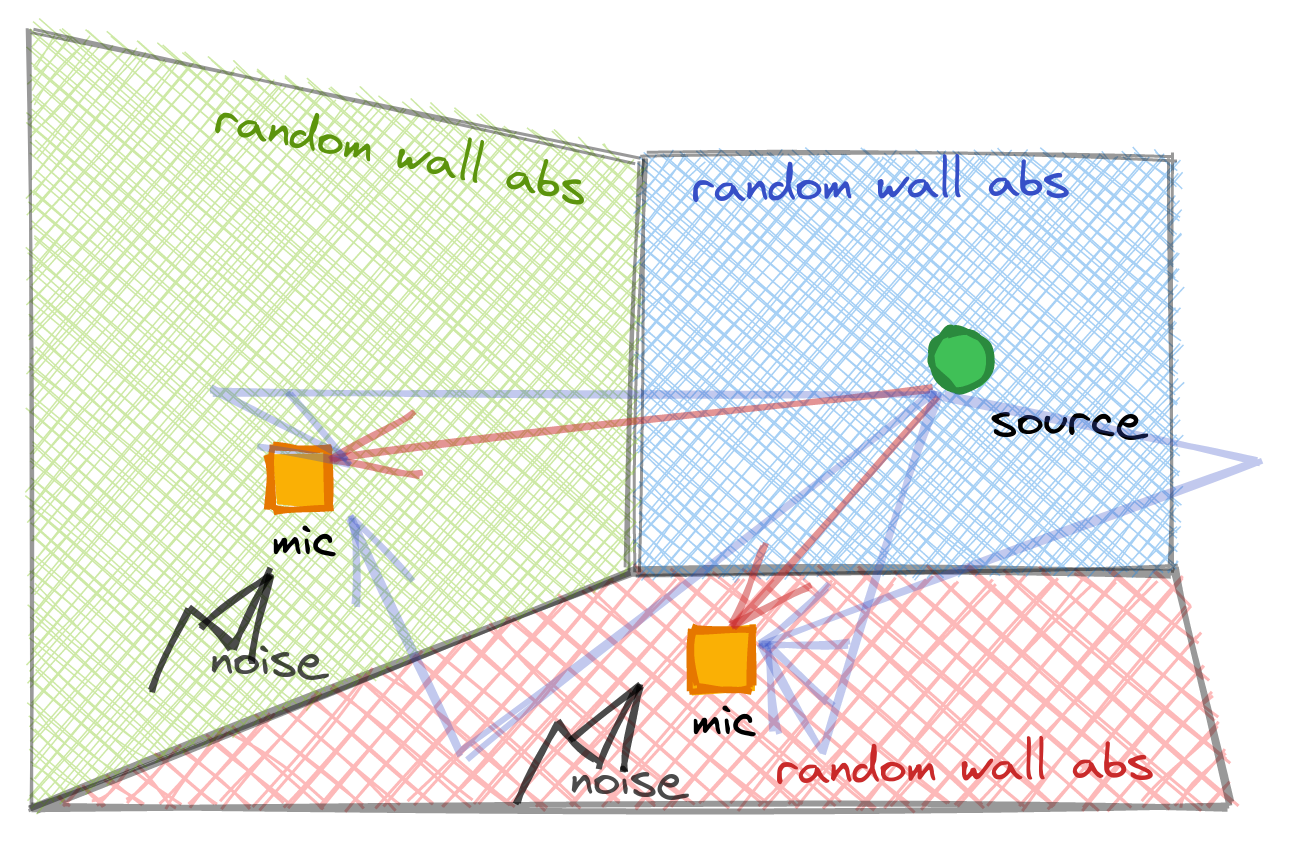
\includegraphics[width=0.9\textwidth]{figures/aer_scenario4.png}
%         \end{column}
%     \end{columns}

%     \pause
%     \begin{block}{Dataset}
%         \begin{itemize}
%             \footnotesize
%             \item $\mathcal{D^{\text{SNR}}}$: $SNR \in [0, 20]$ dB, $\text{RT}_{60} = 400$ ms
%             \item $\mathcal{D^{\text{RT60}}}$: $\text{RT}_{60} = [100, 1000]$ ms, $SNR = 20$ dB
%         \end{itemize}
%     \end{block}

%     \pause
%     \begin{block}{Metrics}
%         \begin{itemize}
%             \item Precision (how many estimated echoes are correct)
%             \item RMSE (error on the correct guess)
%         \end{itemize}
%     \end{block}

% \end{frame}


% \begin{frame}{Error per Dataset/Signal while recovering 7 echoes}

%     \begin{center}
%         \begin{overpic}[width=0.8\textwidth]{figures/e_k-7_thr-2_bns_crocco_blaster.pdf}
%             \put (102, 48){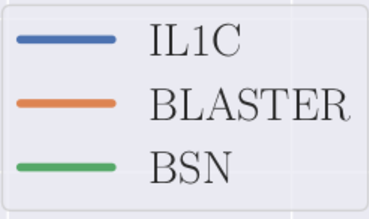
\includegraphics[width=5em]{figures/legend.pdf}}
%         \end{overpic}
%     \end{center}

%     \begin{center}
%         \textcolor{mygreen}{\cmark{Lower RMSE}} \qquad
%         \textcolor{mygreen}{\cmark \, \parbox{8.5em}{Robustness\\
%         to SNR and $\text{RT}_{60}$}} \qquad
%         \textcolor{myred}{\xmark \, \parbox{8em}{Source signal\\dependent}}
%     \end{center}

% \end{frame}




% \begin{frame}<1>[label=echoes]{Performance per \# of echoes}
%     \begin{figure}[t!]
%     \centering
%         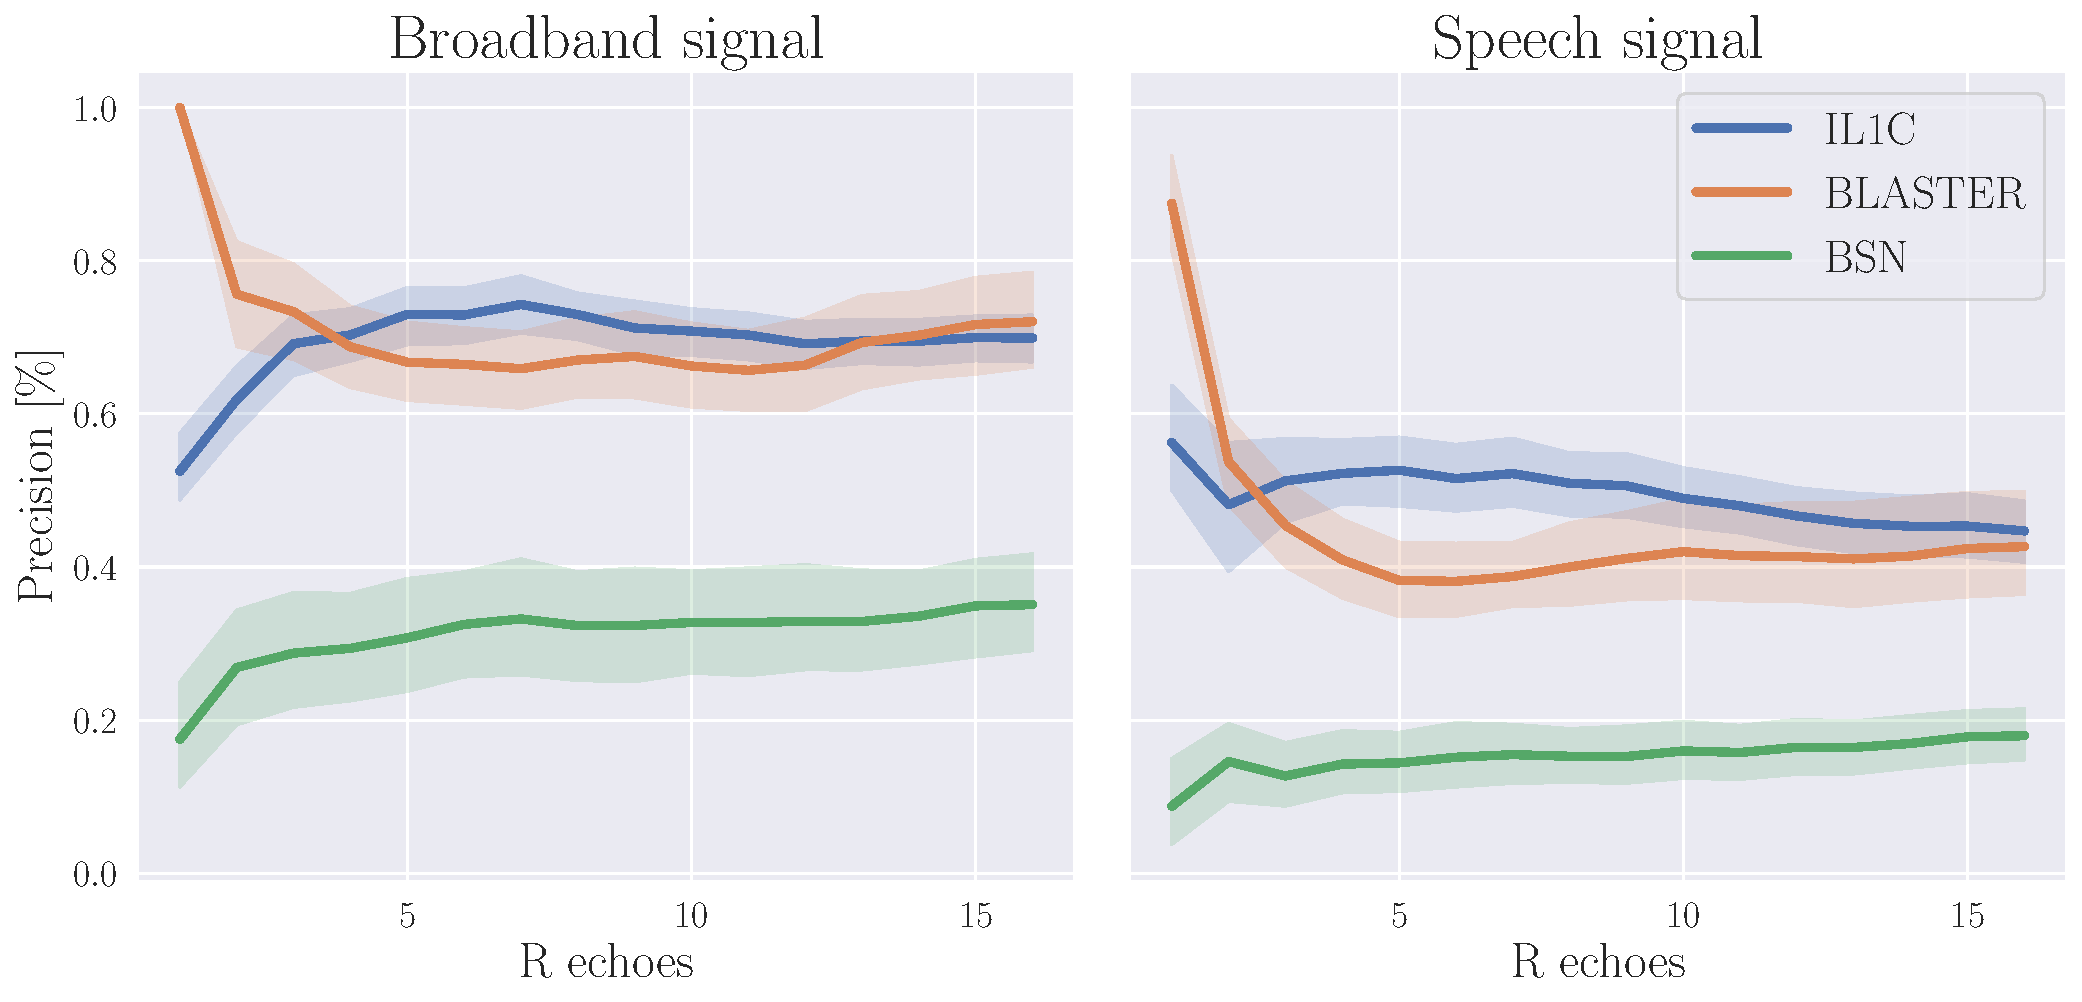
\includegraphics[width=\linewidth]{figures/p_k-7_thr-2_bns_crocco_blaster-peak_withRechoes.pdf}
%         \caption{$\text{RT}_{60} = 400$ ms and SNR = 20 dB.}
%     \end{figure}

%     \begin{center}
%         \textcolor{myred}{\xmark \: \parbox{8em}{Sensitive\\to \# echoes}}
%         \textcolor{myred}{\xmark \: \parbox{8em}{Sensitive\\source signal}}
%         \only<1>{
%         \textcolor{mygreen}{\cmark \: \parbox{8em}{Good\\for 2 echoes}}
%         }
%         \only<2>{
%         \textcolor{mygreen}{
%         \cmark \: \parbox{8em}{Good\\for 2 echoes
%                                     \\\cite{scheibler2018separake,di2019mirage}}}
%         }
%     \end{center}

% \end{frame}

% \againframe<2>{echoes}

% % \subsection{Interim conclusion (2/4)}

% % \begin{frame}{Interim conclusion (2/4)}
% %     \begin{block}{on Acoustic Echo Retrieval:}
% %         \begin{itemize}
% %             \item Most of the literature is on Passive and RIR-based, with on-grid approaches
% %             \item On-grid approaches suffers by the off-grid nature of the echoes (complexity, sampling)
% %         \end{itemize}
% %     \end{block}

% %     \begin{block}{on \blaster:}
% %         \begin{itemize}
% %             \item[\cmark] off-grid parameter-free which exploit dirac closed-form model (non negativity and sparsity)
% %             \item[\cmark] smaller RMSE due to super-resolution, better for small \# of echoes
% %             \item[\xmark] source dependent and on number of echoes
% %             \item[\xmark] validate only on synthetic data
% %             \item[$\rightarrow$] Multichannel and RTF-based extention
% %         \end{itemize}
% %     \end{block}

% %     \begin{block}{on \lantern:}
% %         \begin{itemize}
% %             \item[\cmark] promising results for first echo estimation
% %             \item[\cmark] direct application for table top application
% %             \item[\xmark] difficult extention
% %             \item[\xmark] need for real data validation
% %             \item[$\rightarrow$] physically-constrained neural network
% %             \item[$\rightarrow$] missing frequencies in the input
% %         \end{itemize}
% %     \end{block}
% % \end{frame}
